\problemname{Pinball}
\illustration{.266}{pinball.jpg}{Image from \href{http://www.flickr.com/photos/amalthea23/5764897559/}{Florence Ivy}}

Maria is quite addicted to pinball. She can shoot the ball to any position at the top of the board,
but she cannot predict where the ball will end when it falls down, because it hits many bumpers on
its way down.

She decided to model the pinball table as line segments and assume that the ball is a point that falls from infinite height. The ball falls straight vertically unless there is a segment immediately below it, in which case it follows the direction of the segment downwards until its end.

As you would expect the segments are closed, that is an endpoint is part of its segment. Pairs of segments do not intersect, not even at endpoints, and none is vertical or horizontal. Segments are not given in any specific order.

\section*{Input}

The first line contains an integer $N$ ($0\leq N \leq 100\,000$), the number of segments. Then $N$ lines follow, each with four integers $x_1$ $y_1$ $x_2$ $y_2$, the coordinates of a segment ($-1\,000\,000 \leq x_i,y_i \leq 1\,000\,000$). The last line contains an integer $x_0$ ($-1\,000\,000 \leq x_0 \leq 1\,000\,000$), the initial $x$-coordinate of the ball.

\section*{Output}

Output a single integer $x_T$, the final $x$-coordinate of the ball.

\begin{figure}[h]
  \centering
  \begin{minipage}{0.3\textwidth}
  \centering
    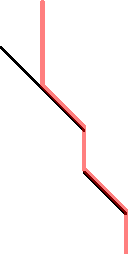
\includegraphics[width=0.58\textwidth]{sample}
    \caption{Sample input 1}
    \label{fig:sample}
  \end{minipage}
  \begin{minipage}{0.3\textwidth}
  \centering
    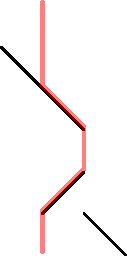
\includegraphics[width=0.58\textwidth]{sample2}
    \caption{Sample input 2}
    \label{fig:sample2}
  \end{minipage}
\end{figure}
